\documentclass{article}
\usepackage{graphicx} % Required for inserting images
\usepackage{verbatim}
\usepackage{amsmath}
\usepackage{algorithmicx}
\usepackage{algpseudocode}
\usepackage{array}
\usepackage{booktabs}


\usepackage{algorithm}



\title{DMA problemset 2}
\author{Daniel Andre Bunckenburg - tvf882@alumni.ku.dk}
\date{February 2025}

\begin{document}

\maketitle

\section{Opgave 1}



\begin{verbatim}

j := n
good := True
while (j > 1 and good) 
    i := j - 1
    while (i >= 1 and good)
        if (A[i] > A[j])
            good := false
        i := i - 1
    j := j - 1
if (good)
    return "Success"
else
    return "failure"

\end{verbatim}



\newpage
\section{Part 2}


\subsection{a}

\begin{figure}[h!]
    \centering
    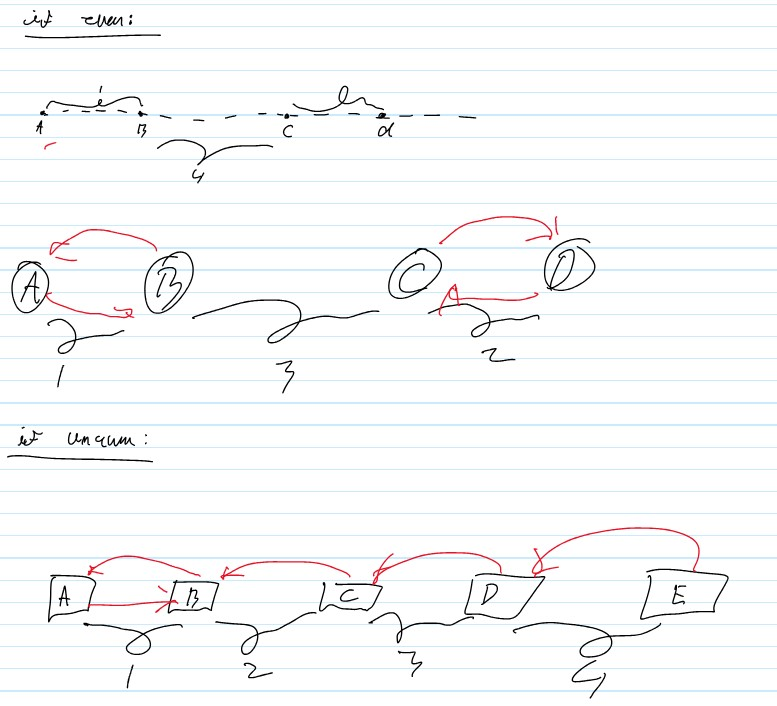
\includegraphics[width=0.8\textwidth]{Figures/figure_1.jpg}
    \caption{Caption for the figure.}
    \label{fig:myfigure}
\end{figure}

If looking at my drawing you see two senarios, the first is if there is an even amount of kids. Then it is possible to position the kids in a way that they are each orther closes, then it is called a mutual 2-cycles and it is possible to that all kids recives a ball, like 
\[
A \to B \quad \text{and} \quad B \to A.
\]

in the orther case

\end{document}
